\documentclass[10pt,a5]{article}

\usepackage[object=vectorian]{pgfornament/latex/pgfornament}
\usepackage{paracol}
\usepackage{setspace}
%\usepackage[landscape]{geometry}
\usepackage[left=1.5cm, right=1.5cm, top = 2cm, bottom = 2cm]{geometry}
%\usepackage{pdfpages}
\usepackage{graphicx}
\usepackage{liturg}
\usepackage{lipsum}

\newcommand \sect[2] {\section*{#1} \switchcolumn \section*{#2} \switchcolumn*}
\newcommand \subsect[2] {\subsection*{#1} \switchcolumn \subsection*{#2} \switchcolumn*}

\newcommand{\sectionlinetwo}[2]{%
  \nointerlineskip \vspace{.5\baselineskip}\hspace{\fill}
  {\resizebox{0.75\linewidth}{1.2ex}
    {\pgfornament[color = #1]{#2}
    }}%
    \hspace{\fill}
    \par\nointerlineskip \vspace{.5\baselineskip}
  }

\setlength\parindent{0pt}

\begin{document}

\massenglish

%\psalmheading{Psalm 42---Judica me}

%\instruct{The priest, signing himself with the Sign of the Cross, says:}

%\leslettrine{C}onf'iteor Deo omnipot'enti, be'at"ae Mar'i"ae semper
%V'irgini, be'ato Micha'eli Arch'angelo, be'ato Jo'anni Bapt'ist"ae,
%sanctis Ap'ostolis Petro et Paulo, 'omnibus Sanctis, et tibi Pater:
%quia pecc'avi nimis congitati'one, verbo, et 'opere:

\begin{paracol}{2}
	\subsect{Concelebrants/Co-celebrantes:}{Musicians/M\'usicos}

	\hspace*{2em}Fr. Nicholas Reynolds, O.P. \\
	\hspace*{2em}Fr. John Restrepo, O.P.

	\switchcolumn

	\hspace*{2em} Soprano: 	Maria Garza \\
	\hspace*{2em} Alto: 	Isabella Anderson \\
	\hspace*{2em} Piano: 	Gray Podolak\\

	\switchcolumn*

	Notes: 
	\begin{itemize}
		\item[$\sim$] (Text between brackets are the translation from the Latin or Portuguese.)
		\item[$\sim$] For each section, an asterisk(*) will indicate which language will be used in the ceremony.
	\end{itemize}

	\switchcolumn


	Notas: 
	\begin{itemize}
		\item[$\sim$] (Texto entre parenteses s\~ao tradu\c{c}\~oes do latim ou ingl\^es.) \\
		\item[$\sim$] Em cada se\c{c}\~ao, um asterisco(*) indicar\`a qual l\'ingua ser\'a usada.
	\end{itemize}

\end{paracol}
\sectionlinetwo{black}{89}
\begin{paracol}{2}
	\subsect{Processional Hymn}{Process\~ao de entrada}

	\hspace*{2em} Jesu, Joy of Man's Desiring - J.S. Bach

	\switchcolumn

	\hspace*{2em} Jesus, Alegria dos Homens - J.S. Bach

	\switchcolumn*

	\subsect{Bridal Entrance}{Entrada da Noiva}

	\hspace*{2em} Canon in D - J. Pachelbel

	\switchcolumn

	\hspace*{2em} Canon em D - J. Pachelbel

	\switchcolumn*

\end{paracol}

\begin{figure}[h]
	\centering
	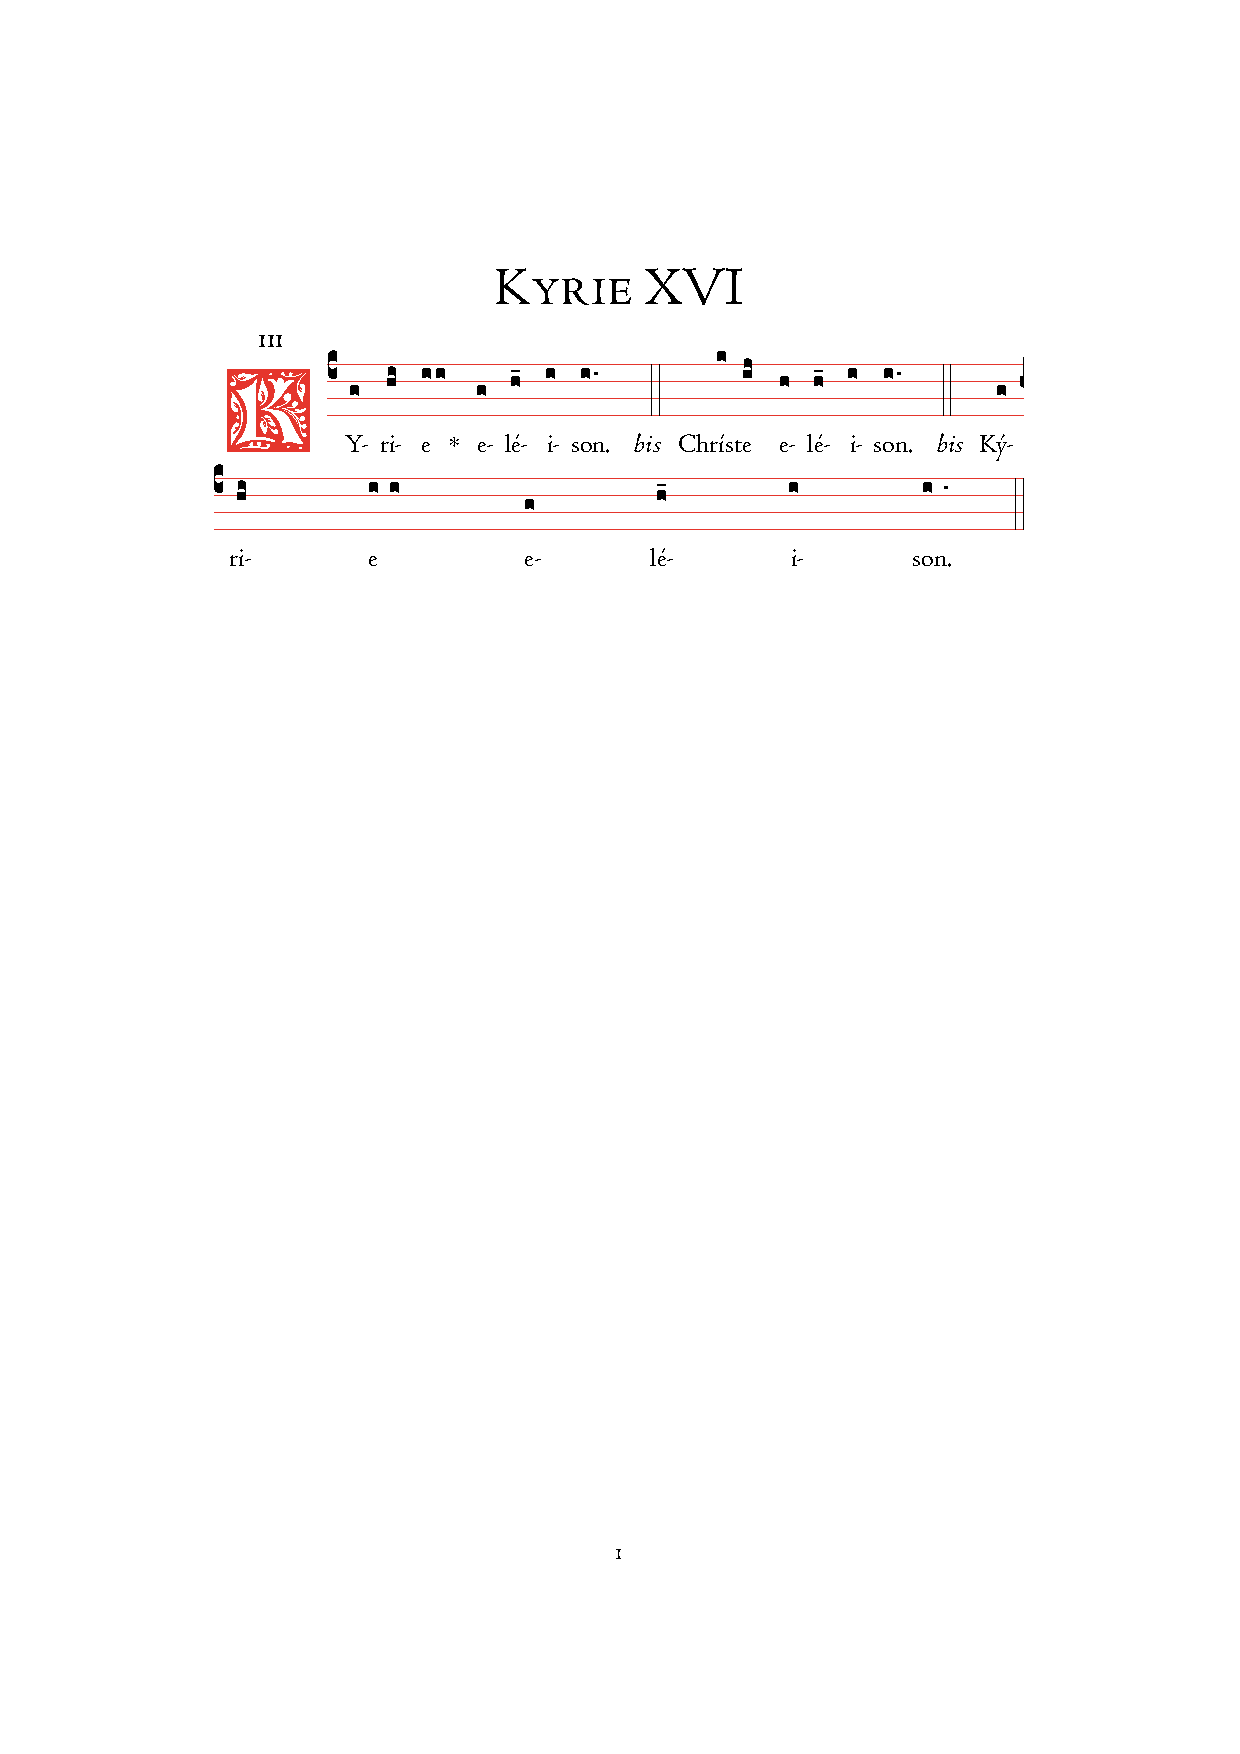
\includegraphics[trim = 35mm 200mm 35.5mm 35mm, clip, width = 0.8\textwidth]{scores/Kyrie-XVI.pdf}
\end{figure}

\begin{paracol}{2}

(Lord, have mercy. Christ, have mercy. Lord, have mercy.)
\switchcolumn
(Senhor, tende piede. Cristo, tende piedade. Senhor, tende piedade)

\switchcolumn*

\subsect{Glory to God}{Gl\'oria}

(Glory to God in the highest,
and on earth peace to people
of good will.
We praise you, we bless you,
we adore you, we glorify you,
we give you thanks for your great
glory,
Lord God, heavenly King, O God,
almighty Father.
Lord Jesus Christ, Only Begotten Son,
Lord God, Lamb of God, Son of the
Father,
you take away the sins of the world,
have mercy on us;
you take away the sins of the world,
receive our prayer;
you are seated at the right hand
of the Father, have mercy on us.
For you alone are the Holy One,
you alone are the Lord,
you alone are the Most High,
Jesus Christ, with the Holy Spirit,
in the glory of God the Father. Amen.)

\switchcolumn

(Gl\'oria a Deus nas alturas e paz na terra aos homens por Ele amados.
 Senhor Deus, Rei dos c\'eus, Deus Pai todo-poderoso:
 n\'os Vos louvamos, n\'os Vos bendizemos, n\'os Vos adoramos, n\'os Vos glorificamos,
 n\'os Vos damos graças, por vossa imensa gl\'oria.
 Senhor Jesus Cristo, Filho Unig\'enito, Senhor Deus, Cordeiro de Deus, Filho de Deus Pai:
 V\'os que tirais o pecado do mundo, tende piedade de n\'os;
 V\'os que tirais o pecado do mundo, acolhei a nossa s\'uplica;
 V\'os que estais \`a direita do Pai, tende piedade de n\'os.
 S\'o V\'os sois o Santo;
 s\'o V\'os, o Senhor;
 s\'o V\'os, o Alt\'issimo, Jesus Cristo;
 com o Esp\'irito Santo na gl\'oria de Deus Pai.
 Am\'em)

 \switchcolumn*

\end{paracol}

\begin{figure}[p]
	\centering
	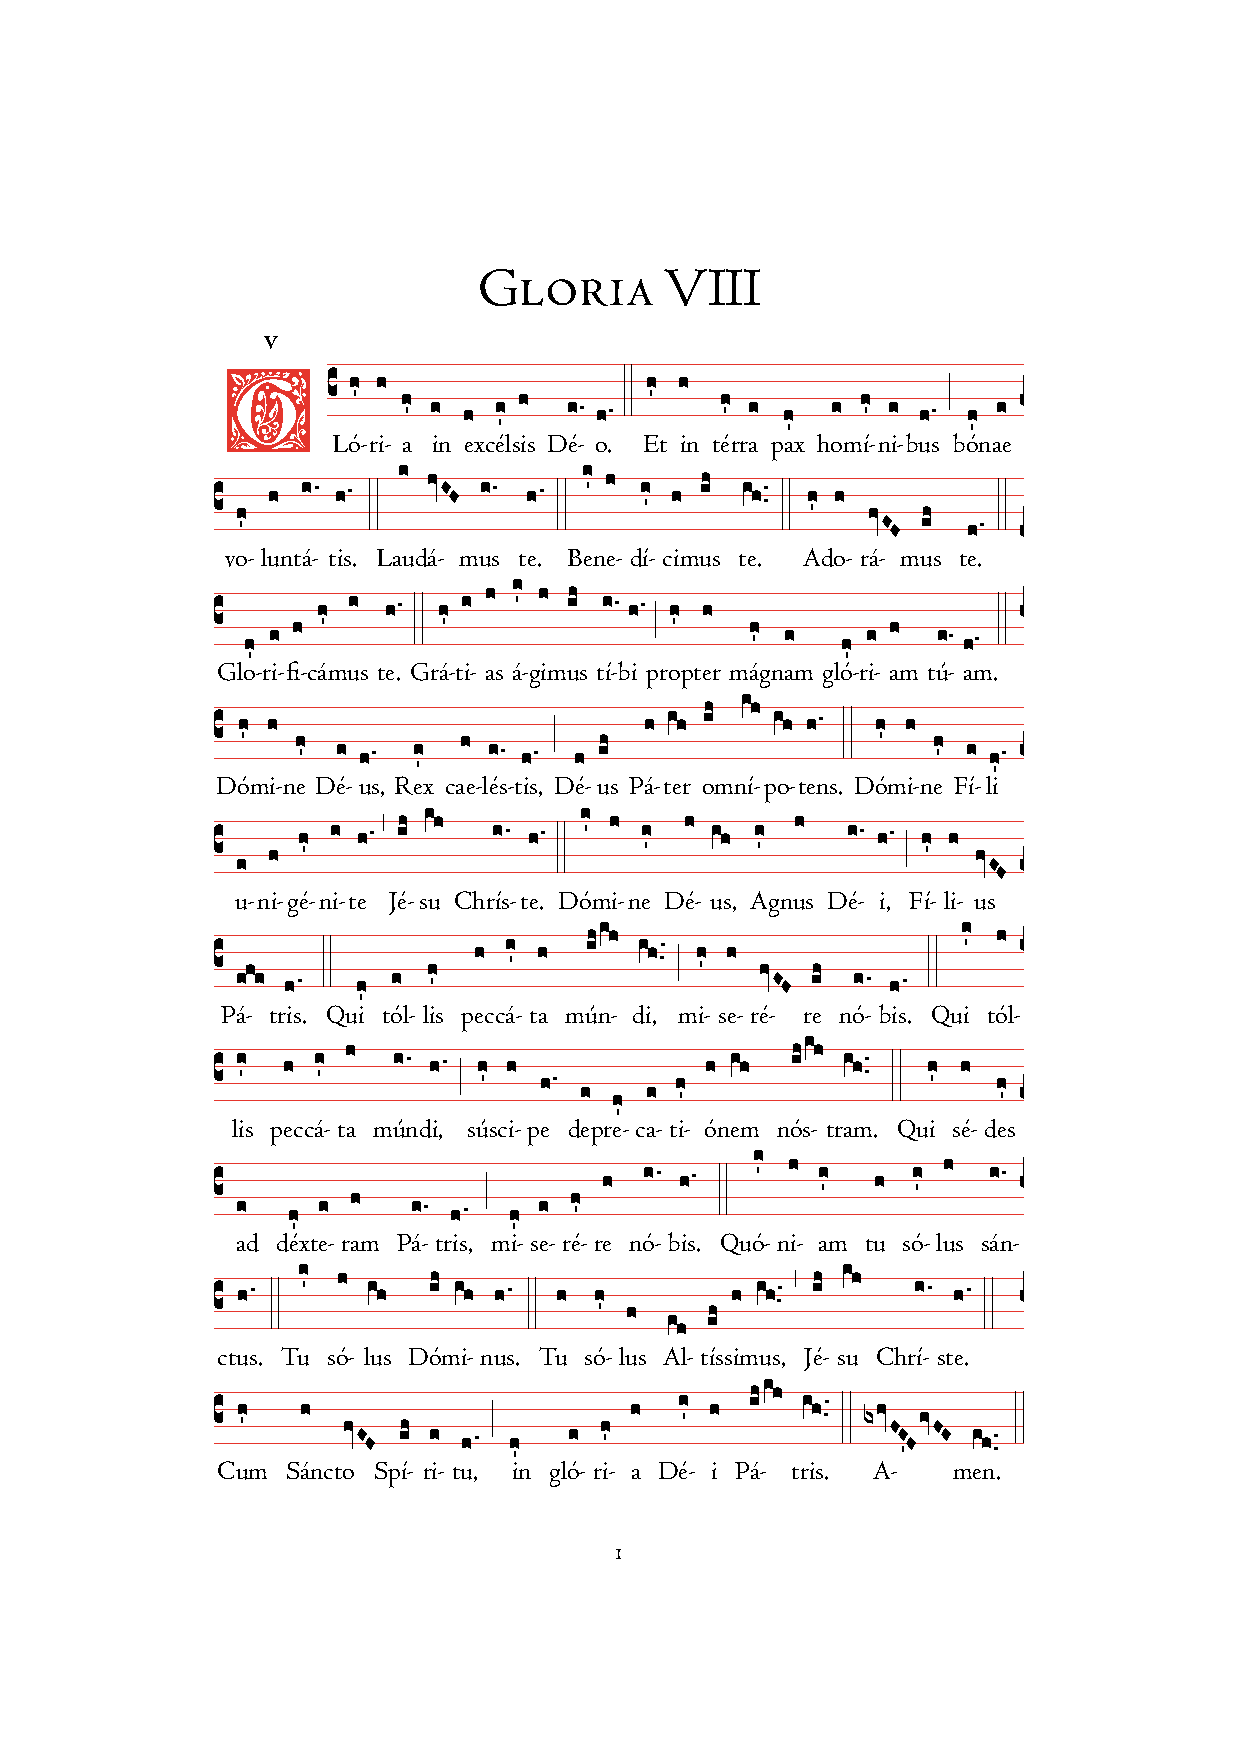
\includegraphics[trim = 35mm 45mm 35.5mm 45mm, clip, width = 0.8\textwidth]{scores/Gloria-VIII.pdf}
\end{figure}

\clearpage

\begin{paracol}{2}

 \sect{Litugy of the Word}{Liturgia da Palavra}

 \sect{First Reading}{Primeira Leitura}

 \textit{Tobit 8:4b-8}

\hspace{2em} A reading from the Book of Tobit

On their wedding night Tobiah arose from bed and said to his wife,
“Sister, get up. Let us pray and beg our Lord to have mercy on
us and to grant us deliverance.”
Sarah got up, and they started to pray
and beg that deliverance might be theirs.
They began with these words:
“Blessed are you, O God of our fathers;
praised be your name forever and ever.
Let the heavens and all your creation
praise you forever.
You made Adam and you gave him his wife Eve to be his help
and support;
and from these two the human race descended.
You said, ‘It is not good for the man to be alone;
let us make him a partner like himself.’
Now, Lord, you know that I take this wife of mine not because
of lust,
but for a noble purpose.
Call down your mercy on me and on her,
and allow us to live together to a happy old age.”
They said together, “Amen, Amen.” \\

%TODO add reader end-of-reading part.
The word of the Lord. \\

\server{Thanks be to God!}

\switchcolumn

\textit{Tobias 8:4b-8}

\hspace{2em} Leitura do Livro de Tobias

Então, Tobias encorajou a jovem com estas palavras: “Levanta-te, Sara, e roguemos a Deus, hoje, amanhã e depois de amanhã. Estaremos unidos a Deus durante essas três noites. Depois da terceira noite, consumaremos nossa união;
porque somos filhos dos santos patriarcas e não nos devemos casar como os pagãos que não conhecem a Deus”.
Levantaram-se, pois, ambos e oraram juntos fervorosamente para que lhes fosse conservada a vida.
Tobias disse: “Senhor, Deus de nossos pais, bendigam-vos o céu, a terra, o mar, as fontes e os rios, com todas as criaturas que neles existem.
Vós fizestes Adão do limo da terra e destes-lhe Eva por companheira.
Ora, vós sa­beis, ó Senhor, que não é para satisfazer a minha paixão que recebo a minha prima como esposa, mas unicamente com o desejo de suscitar uma posteridade, pela qual o vosso nome seja eternamente bendito”.
E Sara acrescentou: “Tende piedade de nós, Senhor; tende piedade de nós e fazei que cheguemos juntos a uma ditosa velhice!”.\\

Palavra do Senhor.\\

 \todos{Gra\c{c}as a Deus!}

 \switchcolumn*

 \subsect{Responsorial Psalm}{Salmo Responsorial}

 \psalmheading{Psalm 128}
 \response{Blest are those who love you, happy those who follow you, blest are those who seek you, O God.}
 \\

 Happy all those who fear the Lord,

 \hspace*{2em}and walk in God's pathway;

You will find what you long for

 \hspace*{2em}the riches of our God.

 \response{Blest are those who love you, happy those who follow you, blest are those who seek you, O God.}
 \\

 Your spouse shall be like a fruitful vine

 \hspace*{2em}in the midst of your home;

 Your children flourish like olive plants

 \hspace*{2em}rejoicing at your table.

 \response{Blest are those who love you, happy those who follow you, blest are those who seek you, O God.}
 \\

May the blessings of God be yours

 \hspace*{2em}all the days of your life,

 May the peace and the love of God

 \hspace*{2em}live always in your heart.

 \response{Blest are those who love you, happy those who follow you, blest are those who seek you, O God.}
 \\


\switchcolumn

\psalmheading{Salmo 127}
\response{Felizes os que temem o Senhor.}
\\
\\

Felizes os que temem o Senhor,  

\hspace*{2em}os que andam em seus caminhos

Poderás viver, então, do trabalho de tuas mãos,

\hspace*{2em}serás feliz e terás bem-estar.

\response{Felizes os que temem o Senhor.}
\\
\\

Tua mulher será em teu lar

\hspace*{2em}como uma vinha fecunda.

Teus filhos em torno à tua mesa 

\hspace*{2em}serão como brotos de oliveira.

\response{Felizes os que temem o Senhor.}
\\
\\

Assim será abençoado 

\hspace*{2em}aquele que teme o Senhor.

De Sião te abençoe o Senhor 

\hspace*{2em}para que em todos os dias de tua vida

\hspace*{2em}possas ver os filhos dos teus filhos.

\response{Felizes os que temem o Senhor.}

 \switchcolumn*

 \subsect{Second Reading}{Segunda Leitura}

 %\lipsum[3]
 \textit{1 Corinthians 12:31-13:8a}

\hspace{2em} A reading from the first letter of Saint Paul to the 

\hspace{2em} Corinthians

Brothers and sisters: Strive eagerly for the greatest spiritual gifts.
But I shall show you a still more excellent way.  
If I speak in human and angelic tongues but do not have love, I am a resounding gong or a clashing cymbal.  And if I have the gift of prophecy and comprehend all mysteries and all knowledge; if I have all faith so as to move mountains, but do not have love, I am nothing.  If I give away everything I own, and if I hand my body over so that I may boast but do not have love, I gain nothing.  
Love is patient, love is kind.  It is not jealous, is not pompous, it is not inflated, it is not rude, it does not seek its own interests, it is not quick-tempered, it does not brood over injury, it does not rejoice over wrongdoing but rejoices with the truth.  It bears all things, believes all things, hopes all things, endures all things.  Love never fails.\\

The word of the Lord. \\

 \server{Thanks be to God.}

 \switchcolumn
 \textit{I Coríntios 12:31-13:8a}

\hspace{2em} Leitura da primeira carta de S\~ao Paulo aos Cor\'intios\\

Aspirai aos dons superiores. E agora, ainda vou indicar-vos o caminho mais excelente de todos.
Ainda que eu falasse as línguas dos homens e dos anjos, se não tiver caridade, sou como o bronze que soa, ou como o címbalo que retine.
Mesmo que eu tivesse o dom da profecia, e conhecesse todos os mistérios e toda a ciência; mesmo que tivesse toda a fé, a ponto de transportar montanhas, se não tiver caridade, não sou nada.
Ainda que distribuísse todos os meus bens em sustento dos pobres, e ainda que entregasse o meu corpo para ser queimado, se não tiver caridade, de nada valeria!
A caridade é paciente, a caridade é bondosa. Não tem inveja. A caridade não é orgulhosa. Não é arrogante.
Nem escandalosa. Não busca os seus próprios interesses, não se irrita, não guarda rancor.
Não se alegra com a injustiça, mas se rejubila com a verdade.
Tudo desculpa, tudo crê, tudo espera, tudo suporta.
A caridade jamais acabará. \\

Palavra do Senhor. \\

 \todos{Gra\c{c}as a Deus!}

 \switchcolumn*

\end{paracol}

\begin{center}

\subsection*{Gospel Acclamation/Aclama\c{c}\~ao ao Evangelho}

Alleluia, Alleluia. Alleluia, Alleluia.

\textit{Everyone who loves is begotten of God and knows God.}

Alleluia, Alleluia. Alleluia, Alleluia.

\end{center}

\begin{paracol}{2}

 \subsect{Gospel}{Evangelho}

 \textit{John 2:1-11}

\hspace{2em} A reading from the holy Gospel according to John 

There was a wedding in Cana in Galilee, and the mother of Jesus was there.
Jesus and his disciples were also invited to the wedding.
When the wine ran short, the mother of Jesus said to him, "They have no wine."
And Jesus said to her, "Woman, how does your concern affect me? My hour has not yet come."
His mother said to the servers, "Do whatever he tells you."
Now there were six stone water jars there for Jewish ceremonial washings, each holding twenty to thirty gallons.
Jesus told them, "Fill the jars with water." So they filled them to the brim.
Then he told them, "Draw some out now and take it to the headwaiter." So they took it.
And when the headwaiter tasted the water that had become wine, without knowing where it came from (although the servants who had drawn the water knew), the headwaiter called the bridegroom
and said to him, "Everyone serves good wine first, and then when people have drunk freely, an inferior one; but you have kept the good wine until now."
Jesus did this as the beginning of his signs in Cana in Galilee and so revealed his glory, and his disciples began to believe in him.\\

{The Gospel of the Lord.}\\

\server{Thanks be to God.}

 \switchcolumn


 \textit{João 2:1-11}

 \hspace{2em} Leitura do Evangelho de Jesus Cristo segundo Jo\~ao

Três dias depois, celebravam-se bodas em Caná da Galileia, e achava-se ali a mãe de Jesus.
Também foram convidados Jesus e os seus discípulos.
Como viesse a faltar vinho, a mãe de Jesus disse-lhe: “Eles já não têm vinho”.
Respondeu-lhe Jesus: “Mulher, isso compete a nós? Minha hora ainda não chegou”.*
Disse, então, sua mãe aos serventes: “Fazei o que ele vos disser”.
Ora, achavam-se ali seis talhas de pedra para as purificações dos judeus, que continham cada qual duas ou três medidas.*
Jesus ordena-lhes: “Enchei as talhas de água”. Eles encheram-nas até em cima.
“Tirai agora” – disse-lhes Jesus – “e levai ao chefe dos serventes”. E levaram.
Logo que o chefe dos serventes provou da água tornada vinho, não sabendo de onde era (se bem que o soubessem os serventes, pois tinham tirado a água), chamou o noivo
e disse-lhe: “É costume servir primeiro o vinho bom e, depois, quando os convidados já estão quase embriagados, servir o menos bom. Mas tu guardaste o vinho me­lhor até agora”.
Esse foi o primeiro milagre de Jesus; realizou-o em Caná da Galileia. Manifestou a sua glória, e os seus discípulos creram nele.\\

{Palavra da salva\c{c}\~ao.}\\
 %\lipsum[3]

 \todos{Gl\'oria a v\'os, Senhor!}

 \switchcolumn*

\end{paracol}

\begin{center}
	\subsection*{Homily/Homilia}
	\subsection*{Celebration of Matrimony/Celebra\c{c}\~ao do Matrim\^onio}
\end{center}
\vspace{1em}

\begin{paracol}{2}

 \subsect{The Creed}{Profiss\~ao de f\'e}
I believe in one God,\\
the Father almighty,\\
maker of heaven and earth,\\
of all things visible and invisible.\\

\switchcolumn

Creio em um só Deus,\\
Pai Todo-Poderoso,\\
criador do céu e da terra,  \\
de todas as coisas visíveis e invisíveis.  \\

\switchcolumn

I believe in one Lord Jesus Christ,\\
the Only Begotten Son of God,\\
born of the Father before all ages.\\
God from God, Light from Light,\\
true God from true God,\\
begotten, not made,\\
consubstantial with the Father;\\
through him all things were made.\\
For us men and for our salvation\\
he came down from heaven,\\
{\color{red}\hspace*{4em}\small\textit{ At the words that follow, up to and including}}\\
{\color{red}\hspace*{6em}\small\textit{``and became man", all bow.}}\\
and by the Holy Spirit was incarnate\\
of the Virgin Mary,\\
and became man.\\
For our sake he was crucified\\
under Pontius Pilate,\\
he suffered death and was buried,\\
and rose again on the third day\\
in accordance with the Scriptures.\\
He ascended into heaven\\
and is seated at the right hand\\
of the Father.\\
He will come again in glory\\
to judge the living and the dead\\
and his kingdom will have no end.\\

\switchcolumn

Creio em um só Senhor, Jesus Cristo,\\
Filho Unigênito de Deus,  \\
nascido do Pai antes de todos os séculos: \\
Deus de Deus, luz da luz,  \\
Deus verdadeiro de Deus verdadeiro,  \\
gerado, não criado,\\
consubstancial ao Pai.  \\
Por ele todas as coisas foram feitas.  \\
E por nós, homens, e para nossa salvação, \\
desceu dos céus: \\
{\color{red}\hspace*{4em}\small \textit{Aqui todos se curvam at\'e as palavras }}\\
{\color{red}\hspace*{6em}\small \textit{``e se fez homem".}}\\
e se encarnou pelo Espírito Santo,  \\
no seio da Virgem Maria, \\
e se fez homem. \\
Também por nós foi crucificado \\
sob Pôncio Pilatos;  \\
padeceu e foi sepultado.  \\
Ressuscitou ao terceiro dia,  \\
conforme as Escrituras,  \\
e subiu aos céus,  \\
onde está sentado à direita \\
do Pai.  \\
E de novo há de vir, em sua glória,  \\
para julgar os vivos e os mortos;  \\
e o seu reino não terá fim.  \\

\switchcolumn

I believe in the Holy Spirit,\\
the Lord, the giver of life,\\
who proceeds from the Father\\
and the Son,\\
who with the Father and the Son\\
is adored and glorified,\\
who has spoken through the prophets.\\

\switchcolumn

Creio no Espírito Santo,  \\
Senhor que dá a vida,  \\
e procede do Pai \\
e do Filho;  \\
e com o Pai e o Filho \\
é adorado e glorificado:  \\
ele que falou pelos profetas.  \\

\switchcolumn*

I believe in one, holy, catholic\\
and apostolic Church.\\
I confess one Baptism\\
for the forgiveness of sins\\
and I look forward to the resurrection\\
of the dead\\
and the life of the world to come. Amen.\\

\switchcolumn

Creio na Igreja, \\
una, santa, católica e apostólica.  \\
Professo um só batismo \\
para remissão dos pecados.  \\
E espero a ressurreição \\
dos mortos  \\
e a vida do mundo que há de vir. Amém.

\switchcolumn*

\end{paracol}

\begin{center}
\subsection*{Offertory/Ofert\'orio - Irish Blessing}
\end{center}

Refrain

May the road rise up to meet you,
May the wind be always with you,
May the sunshine warm you always
til we meet again.\\

Verses

1. May the rain fall softly on you,
May the hand of God uphold you.

2. Christ before you, Christ behind you,
Christ beneath you, Christ above you.

3. Christ to shield you, Christ be with you,
Christ be with you now and always.

4. Christ in every eye that sees you,
Christ in every ear that hears you.

5. Christ in every heart that knows you,
Christ in every word that speaks of you.

\begin{figure}[h!]
	\centering
	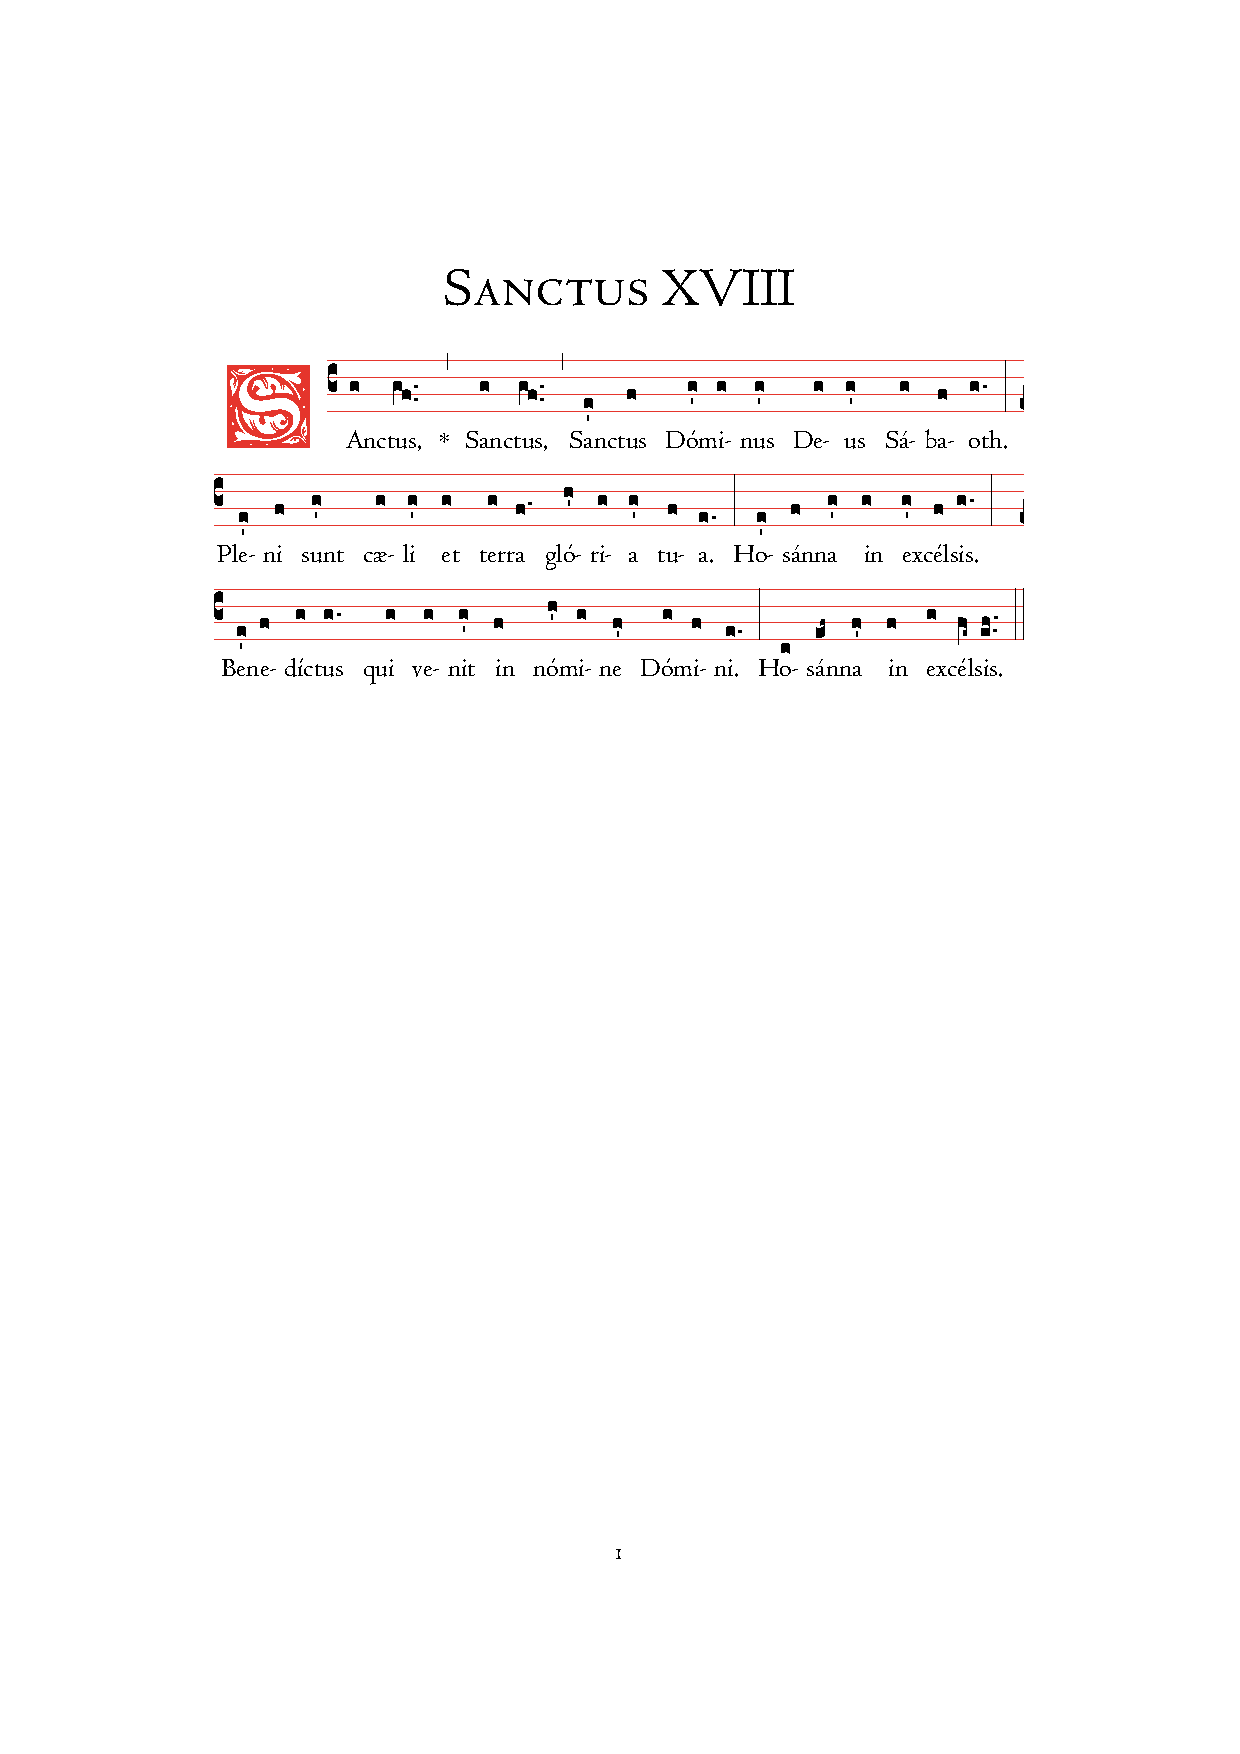
\includegraphics[trim = 35mm 175mm 35.5mm 45mm, clip, width = 0.8\textwidth]{scores/Sanctus-XVIII.pdf}
\end{figure}

\begin{paracol}{2}

(Holy, holy, holy lord God of hosts.
Heaven and earth are full of your glory.
Hosanna in the highest.
Blessed is he who comes in the name of the Lord.
Hosanna in the highest.)

\switchcolumn
(Santo, Santo, Santo, Senhor Deus do universo! O céu e a terra proclamam a vossa glória. 
Hosana nas alturas! Bendito o que vem em nome do Senhor! Hosana nas alturas!)

\switchcolumn*

\subsect{Eucaristic Prayer}{Ora\c{c}\~ao Eucar\'istica}

...

\priest{The mystery of faith!}

\switchcolumn

...

\priest{Eis o mist\'erio da f\'e!}

\end{paracol}

\clearpage

\begin{figure}[h!]
	\centering
	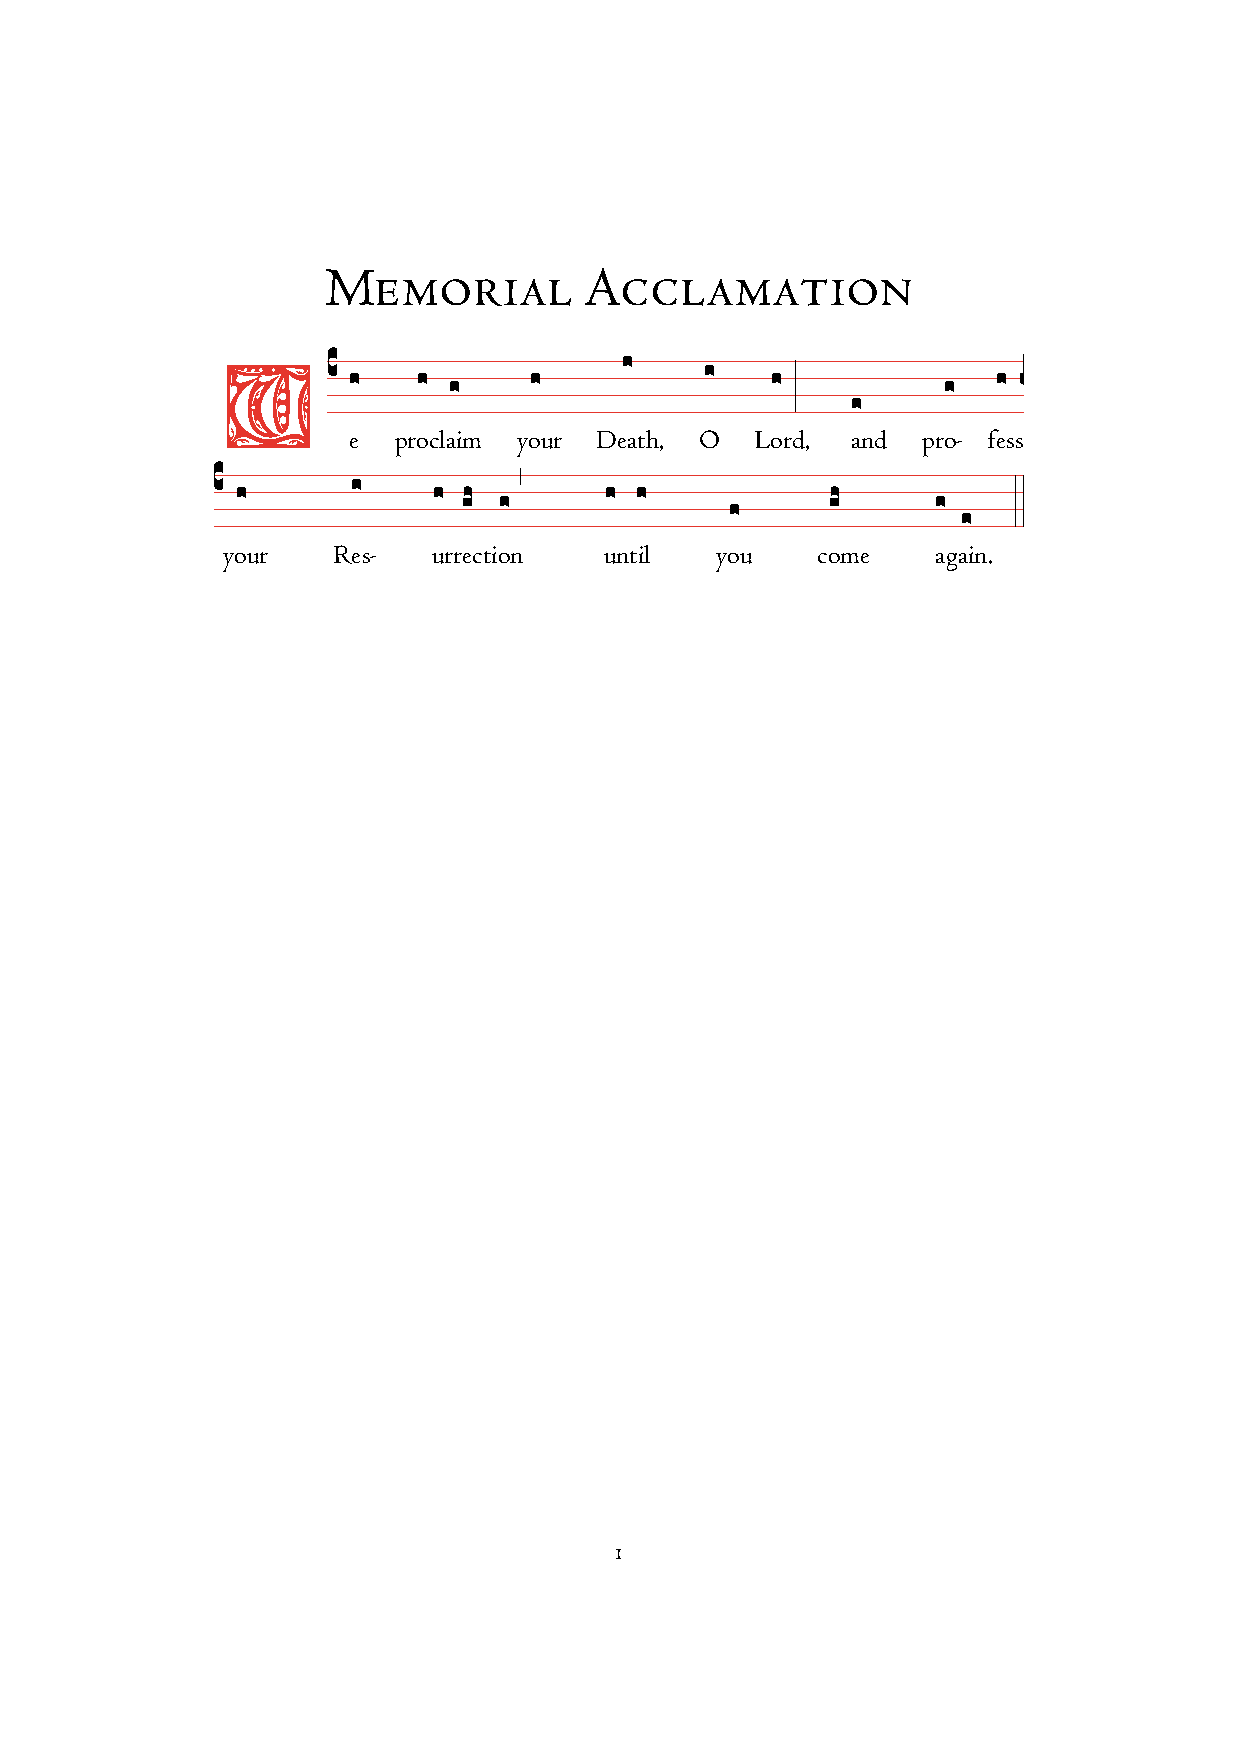
\includegraphics[trim = 35mm 200mm 35.5mm 45mm, clip, width = 0.8\textwidth]{scores/Memorial-Acclamation.pdf}
\end{figure}

\begin{paracol}{2}

\switchcolumn

(Anunciamos, Senhor, a vossa morte e proclamamos a vossa ressurreição. Vinde, Senhor, Jesus!)

\end{paracol}

\begin{figure}[h!]
	\centering
	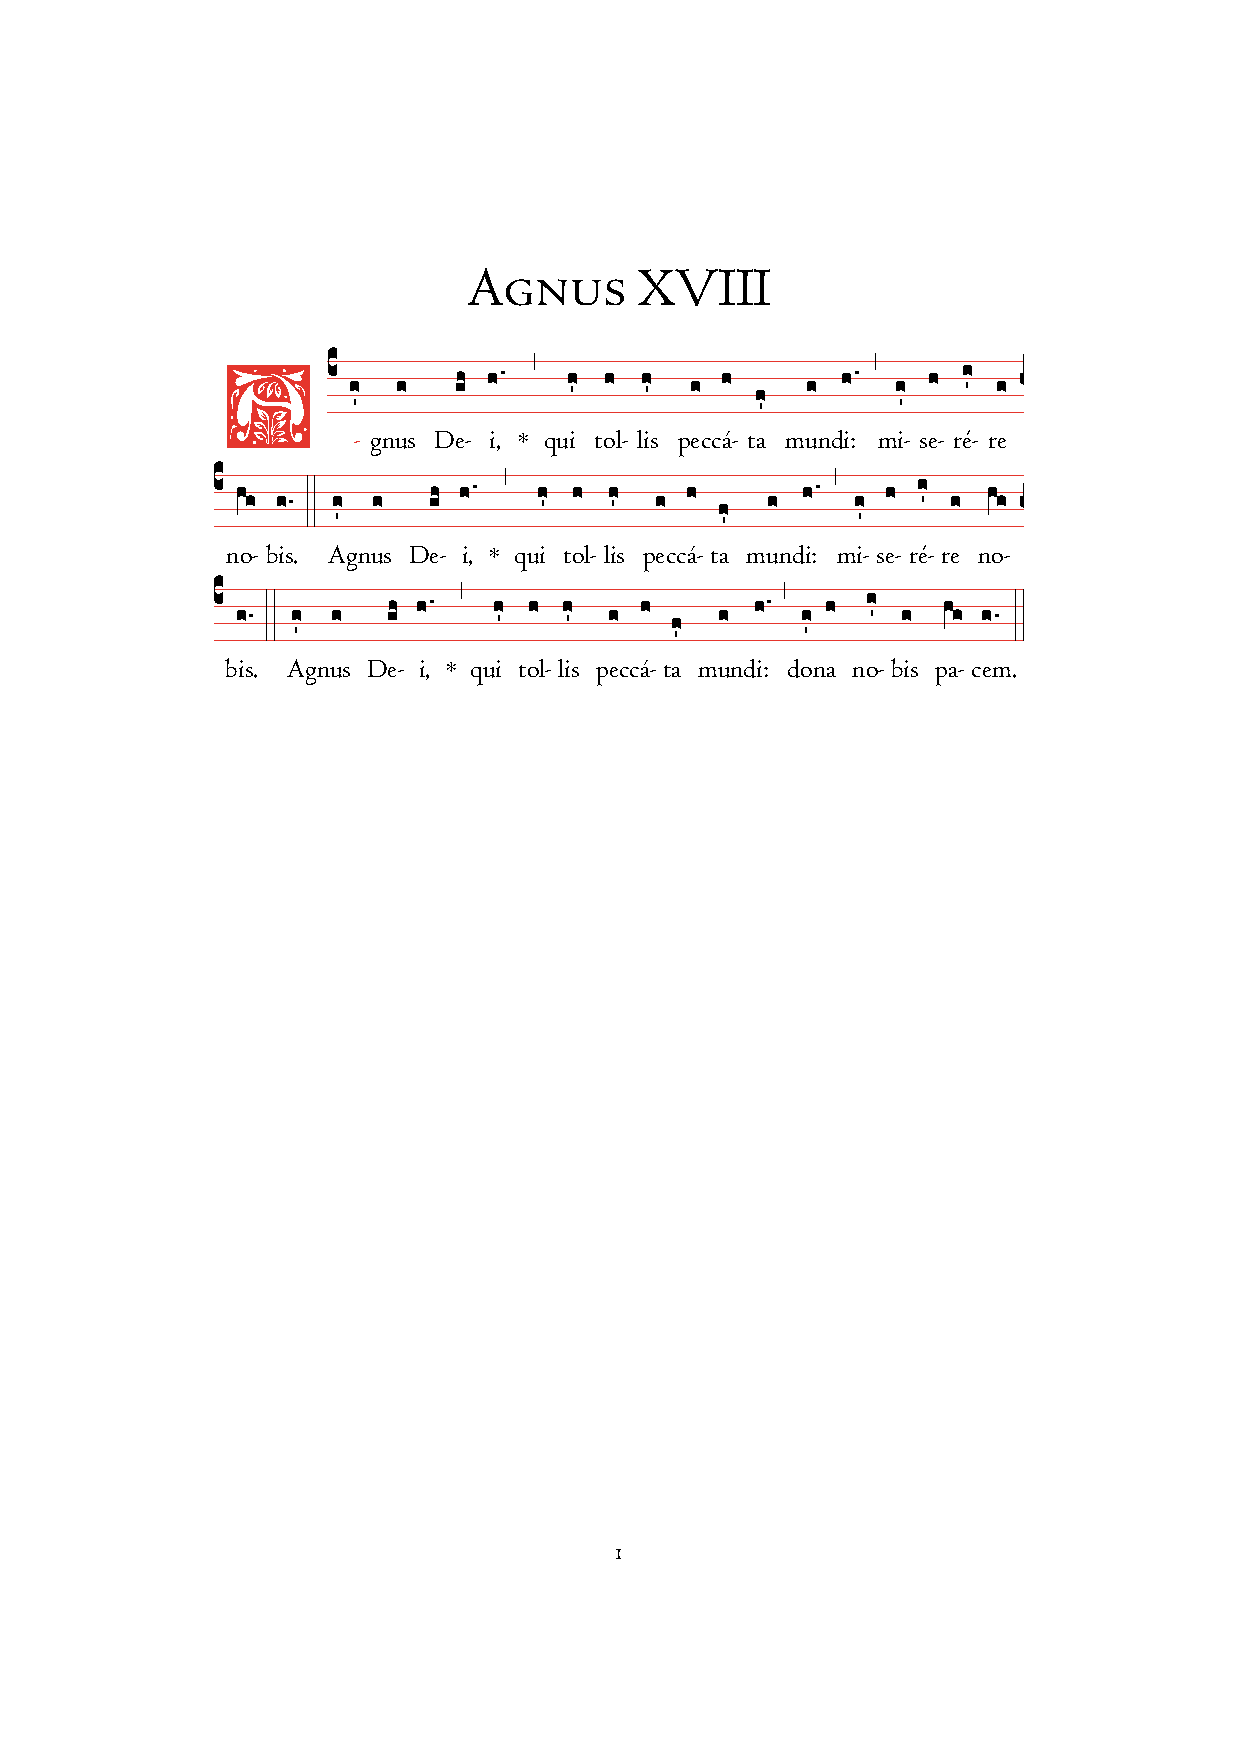
\includegraphics[trim = 35mm 175mm 35.5mm 35mm, clip, width = 0.8\textwidth]{scores/Agnus-XVIII.pdf}
\end{figure}

\begin{paracol}{2}

(Lamb of God, you take away the sins of the world, have mercy on us.
Lamb of God, you take away the sins of the world, have mercy on us.
Lamb of God, you take away the sins of the world, grant us peace.)

\switchcolumn

(Cordeiro de Deus, que tirais o pecado do mundo, tende piedade de nós.
Cordeiro de Deus, que tirais o pecado do mundo, tende piedade de nós.
Cordeiro de Deus, que tirais o pecado do mundo, dai-nos a paz.)

\switchcolumn*

\end{paracol}

\begin{center}
\subsection*{Communion/Comunh\~ao \\ Lord, You Have Come/A Barca \ \ \ \ \ \ \ \ \ \ \ \ \ \ \ \ \   }
\end{center}

Lord, you have come to the seashore,
neither searching for the rich nor the wise,
desiring only that I should follow.\\

O, Lord, with your eyes set upon me,
gently smiling, you have spoken my name;
all I longed for I have found by the water,
at your side, I will seek other shores.\\

Tu sabes bem que em meu barco
Eu não tenho nem ouro nem espadas
somente redes e o meu trabalho.\\

Senhor, tu me olhaste nos olhos,
a sorrir, pronunciastes meu nome.
Lá na praia, eu larguei o meu barco,
junto a Ti buscarei outro mar...\\

Lord, take my hands and direct them.
Help me spend myself
in seeking the lost,
returning love for the love you gave me.\\

O, Lord, with your eyes set upon me,
gently smiling, you have spoken my name;
all I longed for I have found by the water,
at your side, I will seek other shores.\\

Senhor, tu me olhaste nos olhos,
a sorrir, pronunciastes meu nome.
Lá na praia, eu larguei o meu barco,
junto a Ti buscarei outro mar...\\

\begin{paracol}{2}

\subsect{Flowers to Mary - song based on Consecration to our Lady prayer}{Flores para Maria - Consagra\c{c}\~ao a Nossa Senhora}

(Oh my Lady, oh my Mother,
I offer myself entirely to you.
And as proof of my filial affection,
I consecrate you this day,
my eyes, my ears, my tongue, my heart:
in one word, my entire being.
Since I am all yours,
oh Good Mother,
keep me and defend me as your child,
and your possession. Amen.)

\switchcolumn

Ó minha Senhora e também minha mãe,
eu me ofereço, inteiramente todo a vós.
E em prova da minha devoção,
eu hoje vos dou meu coração.

Consagro a vós meus olhos, meus ouvidos, minha boca.
Tudo o que sou, desejo que a vós pertença.
Incomparável mãe, guardai-me, defendei-me,
como coisa e propriedade vossa, amém.

\switchcolumn*

\subsect{Recessional - O God Beyond All Praising}{Canto Final - Tradu\c{c}\~ao}

O God beyond all praising,\\
We worship you today\\
And sing the love amazing\\
That songs cannot repay;\\
For we can only wonder\\
At every gift you send,\\
At blessings without number\\
And mercies without end:\\
We lift our hearts before you\\
And wait upon your word,\\
We honor and adore you,\\
Our great and mighty Lord.\\
\\
Then hear, O gracious Savior,\\
Accept the love we bring,\\
That we who know your favor\\
May serve you as our king;\\
And whether our tomorrows\\
Be filled with good or ill,\\
We'II triumph through our sorrows\\
And rise to bless you still:\\
To marvel at your beauty\\
And glory in your ways,\\
And make a joyful duty\\
Our sacrifice of praise.\\

\switchcolumn

\'O Deus, que excede todo louvor,\\
n\'os Vos adoramos neste dia\\
e cantamos o amor admir\'avel \\
que as can\c{c}\~oes n\~ao podem retribuir;\\
pois 'o podemos nos maravilhar \\
com cada dom que concedeis;\\
com ben\c{c}\~aos sem n\'umero \\
e miseric\'ordias sem fim.\\
Elevamos nossos cora\c{c}\~oes a V\'os\\
e esperamos em Vossa palavra,\\
Vos honramos e adoramos,\\
nosso grande e poderoso Senhor.\\
\\
Escutai, \'o bondoso Salvador, \\
e aceitai o amor que ofertamos,\\
para que, tendo recebido vosso favor,\\
possamos servir-Vos como nosso Rei.\\
E quer sejam nossos amanh\~as \\
repletos de bens ou males,\\
triunfaremos em meio \`as dores \\
e nos levantaremos para Vos bendizer,\\
maravilhar-nos com Vossa beleza \\
e glorificar os Vossos caminhos,\\
e transformar em alegre dever \\
o nosso sacrif\'icio de louvor.\\

\switchcolumn*

\end{paracol}

%\greatfeast{Feria Quinta in Cena Domini}{I}

%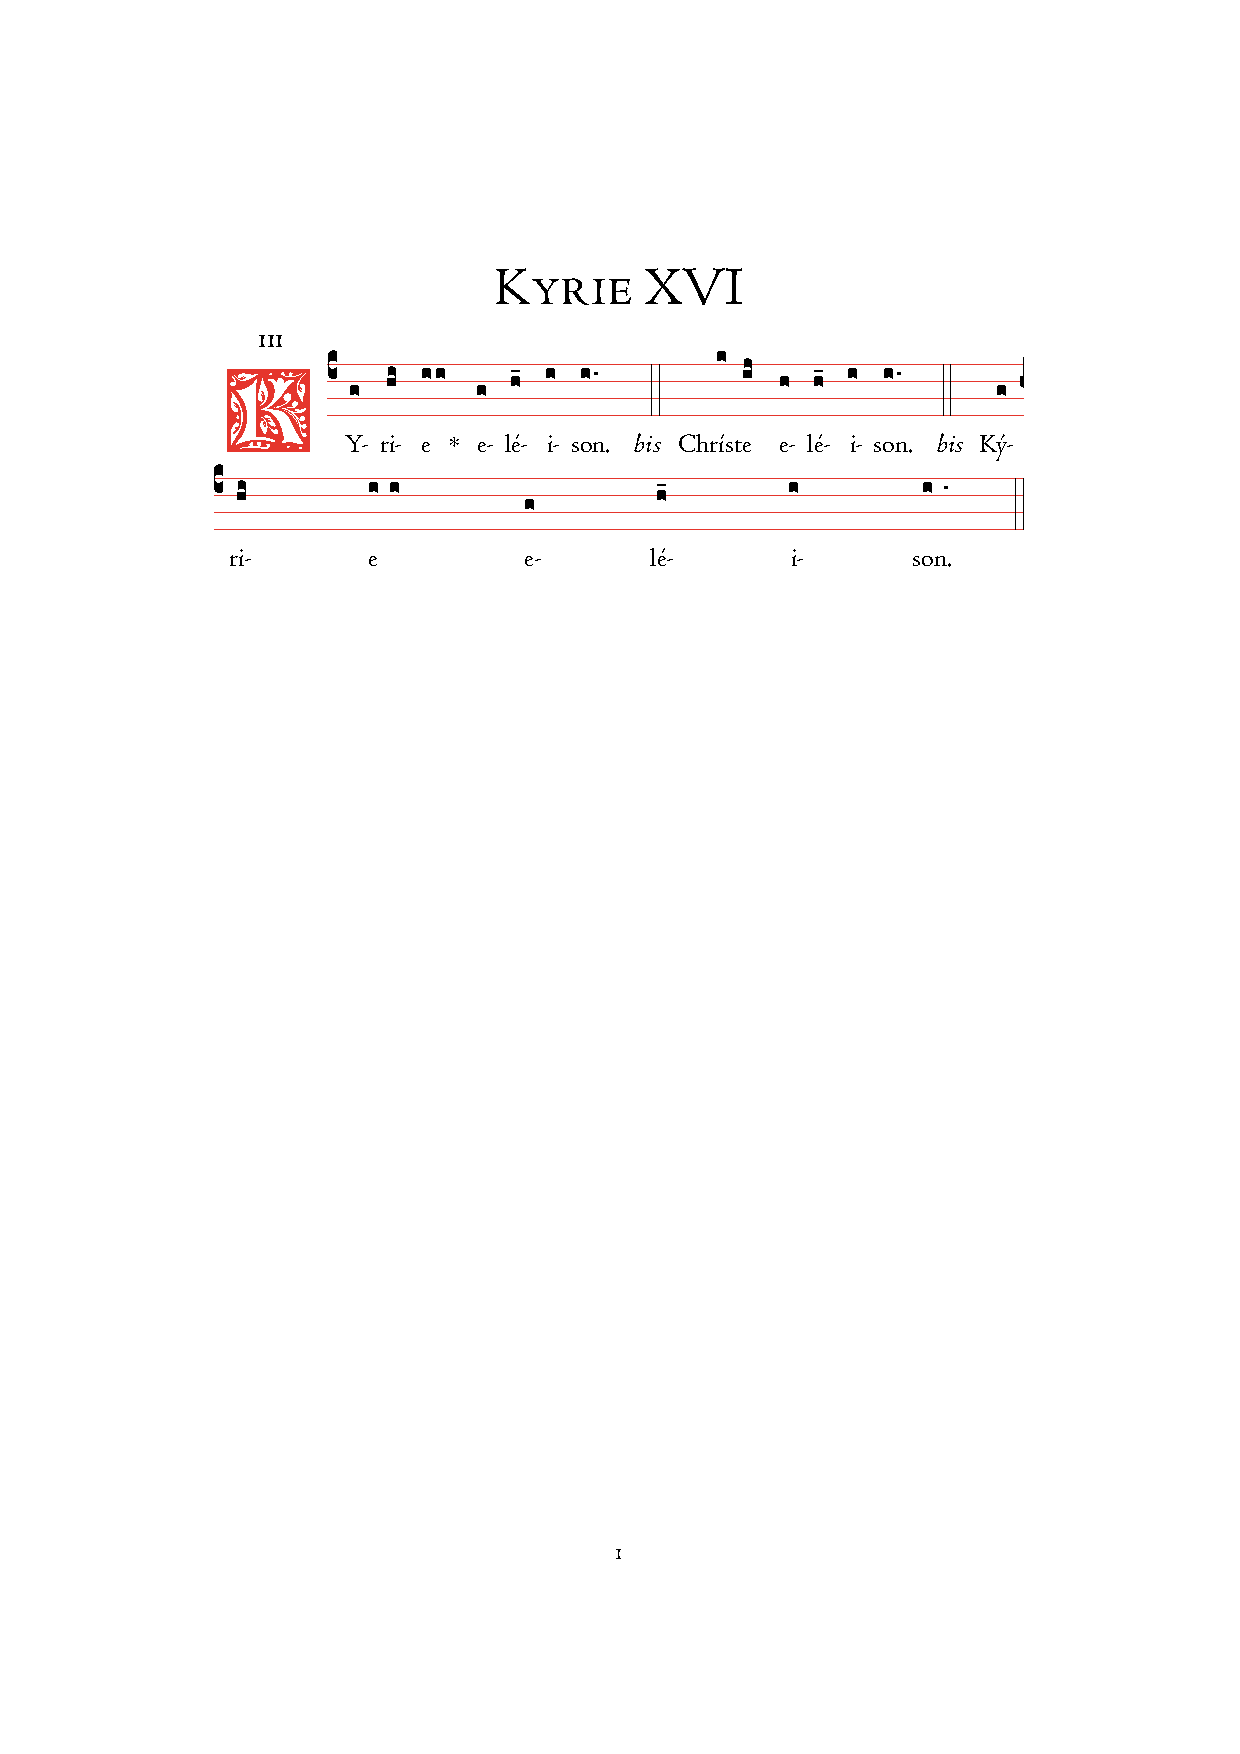
\includepdf[pages=-,pagecommand={},width=\textwidth, trim = 35mm 200mm 20mm 45mm, clip]{scores/Kyrie-XVI.pdf}
\end{document}
